\section{Overview of the \sysname{} System}
\label{sec:overview}

This section provides an overview of \sysname{},
a system that assists developers in partitioning \java{} applications,
by combining \sgx{} hardware protection and \java{} analysis tools.
%with hardened security from both \sgx{}'s security guarantees and 
%\java{}'s safety features.
%% dep
%We will also discuss the threat model assumed in the design of \sysname{}.

\begin{comment}

%\begin{figure}[t!]
%	\centering
%	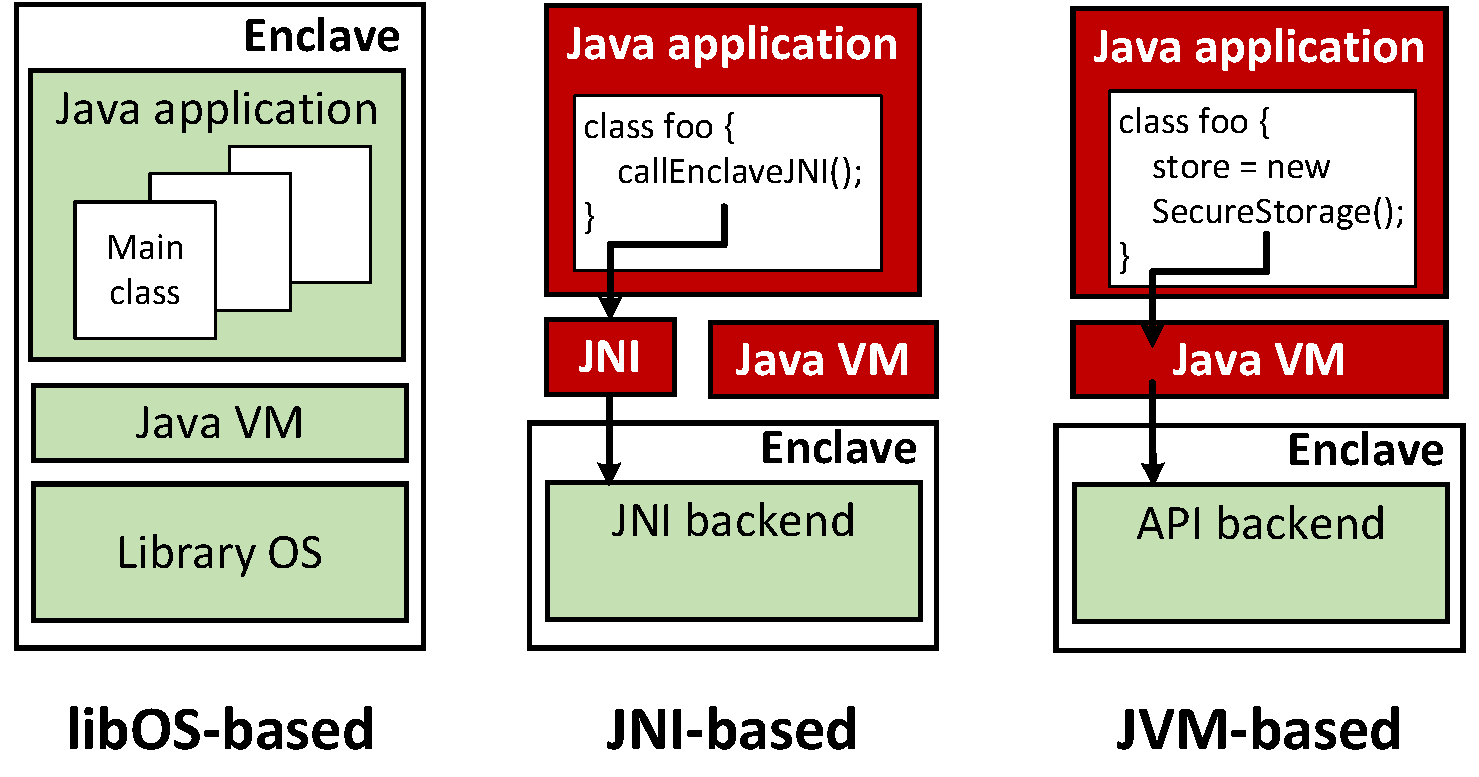
\includegraphics[width=\linewidth]{figures/alternatives.pdf}
%	\footnotesize
%	\caption{Alternative approaches to access \sgx{} hardware protection from \java{} applications.
%		The {\em libOS-based} approach runs the whole \java{} applications in the enclaves. 
%		The {\em JNI-based} approach uses JNI to run the security sensitive operations inside the enclaves.
%		The {\em \jvm{}-based} approach requires the \jvm{} to provide APIs to support common use cases of the enclaves.
%		Green (light) boxes are trusted components and red (dark) boxes are untrusted.
%	}
%	\label{fig:alternatives}
%\end{figure}

There are multiple approaches to access \sgx{} hardware from \java{} applications as illustrated in Figure~\ref{fig:alternatives}. Firstly, the whole \java{} application can run with the \jvm{} inside the enclaves,
using a \sgx{} like Haven~\cite{baumann14haven}({\em libOS-based}).
Secondly, the untrusted components of \java{} application
can run with the \jvm{} outside the enclaves, and a JNI wrapper can communicate
with the trusted component written in native language running inside the enclave like ~\cite{vc3}({\em JNI-based}). 
However,the JNI-based approach requires developers to have the knowledge of
enclave implementation, and loses the language protection of \java{} inside the enclaves.
A more plausible approach is to provide enclave-backed APIs
from the \jvm{},
to support common use cases ({\em \jvm{}-based})), such as a secure key-value store~\cite{vc3}.
Although the \jvm{}-based approach can save the application developers' effort
of implementing isolated components,
the use cases is limited to the pre-defined operations provided by the \jvm{} or the companion frameworks.
Because the backend implementation (isolated components and untrusted interfaces) in the \jvm{}-based approach is the same as the JNI-based approach,
the same language restriction also applies here. 

\end{comment}

\subsection{Design and Features}

\sysname{} consists of a \staticphase{} tool (\statictool{}) and a \dynamicphase{} framework (\dynamicframework{}):
%to help 
%developers to partition \java{} applications.

\paragraph{Partitioning \java{} applications into enclaves (\statictool{})}
To cleanly partition \java{} applications into
 trusted and untrusted components,
 \sysname{} provides a \staticphase{} tool called \statictool{}
%\fixmedp{I recommend naming each component: ``Shredder'' vs. ``the Civet design-time tool''} 
 to automate partitioning.
 In a \sysname{} partition, there are three types of classes.
 First, the developer will identify trusted classes that must execute
 exclusively in the enclave, called an entry class.
 \statictool{}  will identify functions and supporting classes that are reachable
 from the enclave.
 The developer will then decide which additional classes can be instantiated
 only in the enclave, which can be instantiated inside and outside of the enclave, and
 which can only be created outside of the enclave---essentially forming a border
 for the partition.
%The developer manually identifies trusted classes that should be placed in the enclave,
%but will still interact with untrusted components.
%These classes are called entry classes for the enclave.
%Based on the list of entry classes, 
%Shredder selects all supporting classes required by the entry classes,
%the minimal supporting classes that the entry classes have dependency against,
 \statictool{} creates a static image of the in-enclave java classes, packaged as a signed JAR file.
 
 \sysname{} partitions at class granularity, but enforces isolation at  object-level.
 In other words, some classes can execute both in and out of the enclave,
 such as a generic container class or the String class; in these cases,
 the runtime isolation granularity is  object-level (whether it is placed
 in the enclave heap or the untrusted heap).
 \sysname{} does not currently remove unused functions from in-enclave classes,
 although this enhancement could be adopted in future work.
  

%The developer can request for other non-sensitive classes or packages to also be included in the enclave JAR file.
%\fixmedp{Can the developer override this if she wants to exclude some packages, or replicate some packages, rather than share them?  What if she wants instances of the same class in and out of the enclave?}


% \fixmebj{Talk about class level partition granularity and object level isolation granularity.}
%\sysname{} asks the developers to identifies the trusted classes that must be isolated in the enclave,
%but interact with the untrusted components.

For most cases, \sysname{} only requires the developers
to identify the entry classes, and, as desired, to annotate declassifiers for information flow tracking (\S\ref{sec:concept:accessing}).
Our goal is to minimize developer effort required to partition the application.
%This approach minimizes the developer effort 
%The design-time tool of \sysname{} largely reduces the cost of partitioning applications into enclaves.

%In \sysname{}, the developer identifies 
%trusted classes that store
%security sensitive data or code. 
%\fixmedp{Can we say something more crisp about the annotation process.  Maybe related it to the Isolated class definition?}
%Based on the developer's annotations,
%the \sysname{} utility \fixmedp{can we name the pieces?}
%automatically partitions the application into two parts:
%an enclave image and the untrusted image of the application. 
%\fixmedp{I thought the partitioning would be more developer-guided.  
%is the partitioning totally automatic?  Can the developer refine?}
%The enclave includes both annotated classes and classes required by 
%the annotated classes. \fixmedp{Is it just a transitive closure dependency analysis?  Is there ever a case where a class is kept out of the enclave?}
%The \sysname{} utility also creates an interface between the untrusted 
%code, entry points for the enclave, and signs a measurement of 
%the trusted components.

%%% The enclave includes only 
%%% the classes required by  that are depended by the marked classes
%%% are included in the enclaves,
%%% to achieve the golden mean of minimizing the TCB and optimizing performance.


%%% \sysname{} provides application developers with a utility that automatically partitions the application into two parts --- 

%%% \sysname{} statically create entry points for the untrusted interface, and signs the measurement of the trusted components. 


%%%  developers 
%%% partition their code, and provides runtime support to securely and 
%%% seamlessly run trusted components in \sgx{}.
\paragraph{Triggering enclave execution for partitioned \java{} classes (\dynamicframework{})}
To seamlessly trigger enclave execution and access in-enclave objects,
\sysname{} provides a \dynamicphase{} framework called \dynamicframework{} to load the partitioned \java{} classes into enclaves.
% and make \sgx{} protection guarantees first class components of the \java{} language.
%When \sysname{} is called to run isolated \java{} components,
\dynamicframework{} creates two \java{} execution environments: 
one in the enclave (\emph{trusted}) and one outside the enclave (\emph{untrusted}), as illustrated in Figure~\ref{fig:synthesis}.
%Both environments have an individual \jvm{}.
The \jvm{} outside the enclave is the default \jvm{}; the \jvm{} inside the enclave is a lightweight \jvm{},
with just enough features to support the trusted components but a smaller TCB.
%The lightweight \jvm{} runs in a an enclave \sgx{}.
%\dynamicframework{} abstracts the low-level semantics of the \sgx{} hardware from the applications.

 
\dynamicframework{} creates an enclave % for the trusted classes
the first time an entry class is instantiated,
or untrusted code calls a static, public method of an entry class.
The \sysname{} framework front-end uses the signed JAR file that
contains all the trusted supporting classes
as the image to verify and load into the enclave.
%(all trusted classes packaged in the same JAR file share one enclave).
Figure~\ref{fig:synthesis} illustrates this process.
%Take the code snippet in Figure~\ref{fig:synthesis} for example.
When the class {\tt Untrusted} instantiates the trusted class {\tt Trusted},
\sysname{} framework creates the enclave,
and instantiates {\tt Trusted} inside the enclave so the execution will be isolated.
%\fixmedp{The class is called Isolated in the figure}


After the trusted classes are instantiated, the untrusted classes can call public methods on the Trusted objects.
Calling a trusted object function from outside the enclave transfers control to the \sysname{} framework back-end, which then 
calls the appropriate method on the object in the enclave---conceptually similar to a remote procedure call, but on the same CPU core.
In the example in Figure~\ref{fig:synthesis}, a call to method {\tt Trusted.process()} from an the {\tt Untrusted} class,
causes entry to the enclave to run the method.
%which transfers control into the enclave.
%The \sysname{} front-end will re-enter the enclave, and the back-end will make the invocation on the correspondent object, with isolation.
%will trigger entry of the enclave, to run the method. 

%We chose to use two \jvm{}s to minimize the risk of the trusted \jvm{}'s integrity 
%being compromised.  The other sensible option might be to 
%run a single \jvm{} in the enclave that also services the untrusted code.
%The risk of running only one \jvm{} in the enclave is that the attack surface for the enclave is considerably
%wider, and there is more risk of attacks on the integrity of the trusted \jvm{} by untrusted code.
%Of course, one can also place the \jvm{} outside of the enclave, but using an untrusted language runtime
%seems dauntingly difficult and is beyond the scope of this paper.




\paragraph{\java{} APIs for accessing enclave features}
\sysname{} provides a \java{} class ({\tt Enclave}) for application developers
to use enclave features, such as attestation and secure provisioning.
For attestation, \sysname{} generates a proof of the enclave integrity signed by the CPU,
with the hardware measurement of the \sysname{} runtime;
the \sysname{} runtime combines this with a measurement of the loaded classes.
For secure provisioning,
\sysname{} can secure a connection with a remote host,
by encrypting the connection and authenticate both sides using attestation.
This class is useful for features such as loading a sensitive class file or transferring
a secret 
from a trusted, remote host.
%\fixmedp{and then load a class file from the remote host?}

\paragraph{Minimizing the enclave footprint.}
By default, Java imports code liberally, on the assumption that unreachable code
will never be loaded or JIT compiled.
The standard runtime library, {\tt rt.jar}, contains more than 17.8 thousand classes, of which only around \roughly{}500 classes are typically loaded.
In the case of an enclave with
remote attestation, all potentially-imported classes must be measured,
which strains limited memory and increases load time.
The Shredder significantly reduces the TCB of code in the enclave by removing irrelevant classes, such as unused utility classes (e.g., {\tt XMLReader}) or  user interface handlers (e.g., {\tt HTTPServer}).
%\fixmedp{I want some concrete EXamples.}
%that are not required to run the code in the enclave.

%A \java{} application often yields a huge TCB, including the \jvm{},
%JNI and loaded classes.
%For example, the \jvmname{} binaries are 40MB in total. 

%\fixmets{these are rough numbers, find out the precise ones}
%On the other hand, the actual classes needed by an application from {\tt rt.jar}
%can be as less as 1,000 classes.
%Majority of the classes provided from {\tt rt.jar},
%--- even though they may never be loaded into the enclave ---
%still remains in the TCB.


%Having unnecessary binaries and classes in the TCB of the enclave
%can aggravate the risk of being attacks.
%First of all, the huge amount of code loaded into the enclave
%increase the opportunity of having gadgets that can be exploited in ROP attacks,  
%which can still happen in the \jvm{} or JNI.
%Even though most of the \java{} classes have static footprint of their supporting classes,
%many of them still dynamically load classes, such as directly calling the class loader, or specifying providers to the \java{} cryptography framework.
%Having huge TCB as \java{} classes in the enclave still intensify
%the risk of attacks, even though \java{} classes are immune to control flow attacks. 

%We further reduce the TCB by removing unused \jvm{} features such as multi-threaded garbage collection and JIT compilers, unused classes from the \java{} standard runtime library, and unused APIs from the \sgx{} and the C standard library.
%\fixmedp{DO NOT JUST REMOVE THIS FIXME WITH ``best effort'' HAND-WAVING!!! I WANT A GODDAM LIST OF EXAMPLE \jvm{} FEATURES COMPILED OUT---to keep the sentence above, you must have a quick list of examples of what you chop out}


\paragraph{Implementation.} \sysname{} is built upon \jvmname{}, using \java{} and JNI.
\sysname{} requires no changes to the default \jvm{} in the host,
but does modify the lightweight \jvm{} inside the enclave.

\subsection{Security Properties}

%\paragraph{Security guarantees.}
\sysname{} provides comparable security properties to an enclave running a static, native binary.
First, \sysname{} maintains code integrity by verifying the signed JAR file that contains all the supporting classes, potentially including classes from the \java{} Standard Library.
All methods and objects of the trusted classes are completely isolated 
%\fixmedp{what does it mean to be strictly isolated?} 
inside the \sgx{} enclave.
The objects returned from isolated methods of trusted classes are only released
from the enclave if the developers explicitly use the \sysname{}'s declassifier API to mark the objects as safe.
%\fixmedp{How does this happen?}

We explain in more detail below how \sysname{} helps developers reduce the enclave's attack surface,
by providing building blocks for tracking information flows within the enclave, code confidentiality, and remote attestation.

%\fixmedp{What about confidentiality?  Remote attestation?  Can we state some properties that prevent the common pitfalls in the previous section?  Right now, we are underselling a bit---feels like you are just dumping java in an enclave}


%The untrusted classes run on a \jvm{} that includes an untrusted, JNI-based
%\sysname{} front-end, which creates the trusted enclave.
%The back-end runs inside the enclave, and includes a minimal \jvm{}
%running on top of a \sgx{}.  This \jvm{} interprets...
%\fixmedp{I'd like to say more here about the isolated class and how this
%works.  I would also mention how the app differentiates when Isolated
%is really in an enclave and when it isnt (i.e. an example 
%of how remote attestation would work}

%\sysname{} automatically generates the ``glue'' code between
%the front and back end. \fixmedp{I might comment a bit more about 
%the semantics when a class is used in both places, and how 
%data moves back and forth, at a high level}

%JNI-based\fixmebj{Is that correct?} \sysname{} infrastructure is divided into the front-end to create enclave, and call one of the entry points in the back-end running inside the enclave. The back-end uses a libOS to run a minimal \jvm{} inside the enclave to interpret and execute the bytecode of the class {\tt Isolated}.
%The front-end detects and intercepts {\tt Isolated} class object creation and {\tt process} method calls on that object in the untrusted \java VM, and seamlessly transitions to and from the back-end to create the instances or execute the method. 


%, and creates mappings for the entry points on each side to expose public and static methods as the untrusted interfaces. 


%Figure~\ref{fig:synthesis} shows how two parts of the application seamlessly
%interact with each other in \sysname{}. 

%\sysname{} transparently handles all the details of accessing \sgx{} hardware,
%for the loaded \java{} applications.

%%% \subsection{Design and Features}

%%% \sysname{} abstracts the low-level semantics of the \sgx{} hardware from the applications and make \sgx{} protection guarantees first class components of the \java{} language.
%%% \sysname{} is a framework that helps \java{} application developers 
%%% partition their code, and provides runtime support to securely and 
%%% seamlessly run trusted components in \sgx{}.
%%% Figure ~\ref{fig:synthesis} shows how two parts of the application seamlessly
%%% interact with each other in \sysname{}. The JNI-based \sysname{} infrastructure is divided into the front-end to create enclave, and call one of the entry points in the back-end running inside the enclave. The back-end uses a libOS to run a minimal \jvm{} inside the enclave to interpret and execute the bytecode of the class {\tt Isolated}.
%%% The front-end detects and intercepts {\tt Isolated} class object creation and {\tt process} method calls on that object in the untrusted \java VM, and seamlessly transitions to and from the back-end to create the instances or execute the method. 

%%% \sysname{} transparently handles all the details of accessing \sgx{} hardware,
%%% for the loaded \java{} applications.
%%% When \sysname{} is called to run isolated \java{} components,
%%% it creates two worlds of \java{} execution --- one is in the enclave and the other is outside the enclave, and creates mappings for the entry points on each side to expose public and static methods as the untrusted interfaces. 
 
\begin{figure}[t!]
\centering
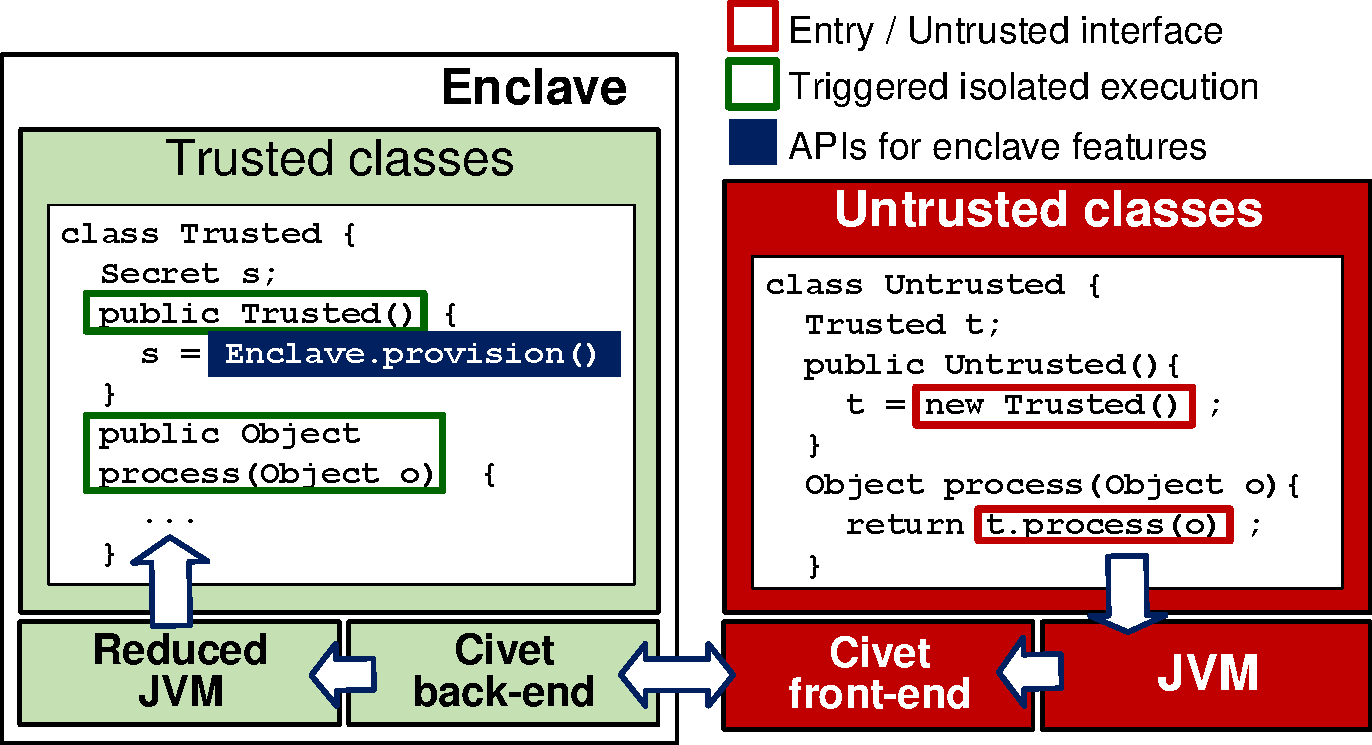
\includegraphics[width=1.0\linewidth]{synthesis-new.pdf}
\footnotesize
\caption{How \sysname{} abstracts the \sgx{} hardware protection for \java{} applications.
When an untrusted class ({\tt Untrusted}) calls the constructor of a trusted class ({\tt Trusted}),
\sysname{} creates the enclave and instantiates in-enclave object.
% class
%inside the enclave. 
The public methods of the {\tt Trusted} class % ({\tt process}) are exported
becomes the enclave interface.
%as the untrusted interface of the enclave, and the invocation of these methods will be re-routed into the enclave.
%\sysname{} also provides APIs for accessing enclave features such as secure provisioning.
}
\label{fig:synthesis}
\end{figure}


%\begin{table*}[t!b!]
\centering
  \begin{tabular}{p{0.05in} >{\raggedright\arraybackslash}p{2.05in} >{\raggedright\arraybackslash}p{4.4in}}
  \toprule
  \multicolumn{2}{l}{\it Security guarantees or features} & {\it The modeling approach applied by \sysname{}} \\
  \midrule
  \midrule
  \multicolumn{3}{l}{\bf Natively provided by the \sgx{} hardware (including the SDK):} \\
  \midrule
  & Isolating security-sensitive components &
  Asking developers to identify multi-level sensitivity, by marking the {\em entry classes}. Complete separation between isolated and untrusted classes.
  \\
  \midrule
  & Secure entry / exit of enclaves &
  Exporting public methods of isolated classes. Arguments are type-checked.
  \\
  \midrule
  & Integrity of the execution environment & 
  Packaging all supporting classes into a signed JAR.
  \\
  \midrule
  & Attestation \& secure provisioning & 
  Providing class {\tt Enclave}, to create secure channels and exchange attestation.
  \\
  \midrule
  \midrule
  \multicolumn{3}{l}{\bf Improvement from combining of \java{} language and the \sgx{} hardware protection:} \\
  \midrule
  & Memory safety \& control flow integrity &
  Naturally provided by \java{} language.
  \\
  \midrule
  & Reducing the enclave TCB &
  Automated partitioning based on class dependencies.
  \\
  \midrule
  & Preventing information flow leakage &
  Tracking information flow in trusted classes, only allow releasing the information if not tainted or declassified by developers.
  \\
  \midrule
  & Code confidentiality & Dynamically loading provisioned classes.
  \\
  \end{tabular}
  
\footnotesize
\caption{
The approaches applied by \sysname{} to model the security guarantees and features of the \sgx{} hardware, and to enhance the security by combining language and hardware protections.
}
\label{tab:features}
\end{table*}


%\subsection{Improvement of Security Properties}


%We discuss each security guarantee or features of the \sgx{} hardware,
%and how they are actually modeled in \sysname{} as follows.
%\fixmebj{Talk about attack surface. Not TCB.}
%partitioning out the minimal supporting classes for the trusted component.
%Beside the classes from the signed JAR file,
%\sysname{} will not load any classes from the host.
%by partitioning out the necessary classes from all the libraries in the developers' class paths, into the enclave image.
%When the enclave is created, the \jvm{} will not load any existing libraries such as {\tt rt.jar} from the host system,
%but instead only search classes in the signed enclave image.
%Minimizing the supporting classes that can be loaded into the enclave
%guarantees that all the classes that are included in the TCB
%are actually required by the isolated components,
%and come from a trusted source such as the developers' execution environment. 


%Note that we do not partition the JNI within the \jvm{} binaries.
%We assume partitioning out the JNI functions that are required by the %isolated classes
%is fully feasible with some manageable efforts.
%Moreover, the \java{} classes can be potentially partitioned at a smaller granularity than the whole classes, such as the methods and fields, which can even further reduce the TCB.
%We leave these potential improvements as future works. 



\paragraph{Information flow control at enclave border}
%The biggest concern for \sgx{} is the threat of secret information leakage. \sysname{} mitigates this threat by leveraging \java{} security solutions
%like information flow control to prevent secret data leaking through implicit as well as explicit flow.
An essential concern for application partitioning is ensuring that 
a bug or vulnerability in the trusted partition does not disclose confidential data
that the partitioning was intended to protect.
Thus, \sysname{} uses information flow control to 
prevent implicit or explicit leaks of sensitive secure provisioned data from the enclave.
%\fixmedp{I assume the developer annotates sensitive data that should not leave, except via a declassifier?}
For classes in the enclave, any confidential data,
such as a private encryption key, is provisioned and protected by \sysname{}.
The \sysname{} runtime framework builds on Phosphor~\cite{bell2014phosphor}
to instrument classes in the enclave to track information flow through the enclave.
At the boundary of the enclave, any variable tainted with a
confidential input cannot leave the enclave unless it is passed through
a declassifier. % or explicitly declassified by the developer using the ~\sysname{} declassification APIs.

\sysname{} does allow references to a confidential object to be
passed out of and into the enclave, using an opaque {\bf proxy object}.
The proxy object can include a serialized and encrypted representation of the data, for literals,
or a reference to an object inside the enclave that can be passed as an argument to a subsequent function.
For JNI functions that make system calls in the enclave, \sysname{} encrypts all data leaving enclave by encrypting at the \sgx{} level.
\sysname{} enforces only confidentiality of the provisioned data, but the infrastructure can be easily extended to ensure data integrity too by propagating taint on enclave inputs.
%\fixmedp{What about integrity?  Does Civet do any checking or taint propagation on inputs?}

We note that these opaque proxy objects strike a reasonable balance between
ease of use and preventing unexpected information flows out of the enclave.
The proxy objects do not contain any indicators about enclave-internal state.
If the same object is returned from multiple functions, each opaque reference is unique, and they cannot be compared for equality.
Similarly, before a literal return value is encrypted, we add a nonce to the plaintext to avoid comparison of the ciphertext.
In the worst case, the untrusted code can leak references via proxy objects, which amounts to a denial-of-service for DRAM---an attack
unavoidable within the threat model of \sgx{}.

%\sysname{} does allow an opaque {\em proxy} object to be returned for 
%guarantee no information flow vulnerabilities
%--- either explicit or implicit
%--- can leak the sensitive information from the enclave.
%\sysname{} filter the information leakage at the enclave border,
%by checking if the the returned values of methods are tainted by the information flow.
%Tainted values are forbidden to leave the enclave,
%but \sysname{} can still make the application proceed, by returning a {\em proxy} of the tainted value (for objects), or encrypt the value (for literals). 

%\sysname{} instruments trusted classes with Phosphor, which provides
%explicit and implicit information flow tracking for \java{} classes.

The \sysname{} prototype supports only shallow declassification.
In other words, objects pointed to by a declassified object are not recursively declassified.


\paragraph{Code Confidentiality}
Code confidentiality is a desirable property for algorithms or code that 
a user wishes to protect, such as a trade secret.
%Code confidentiality can be a desired feature for some developers
%if they wish not to disclose their algorithms.
With \sgx{}, the hardware-level code integrity mechanism is based on a cryptographic
signature of a static binary in plaintext.
\sysname{} can execute confidential code with a dynamic loader that can 
load encrypted classes from remote, trusted hosts.
The remote host uses \sgx{}'s remote attestation features to validate the integrity of the \sysname{} enclave.

%For enclaves that load static binaries,
%code confidentiality is difficult because \sgx{} enclave must load initial code in plaintext, not in encrypted form.


%natively provides code confidentiality by allowing the applications to dynamically load classes
%provisioned from remote, trusted hosts.

%\paragraph{Attestation and Secure Provisioning}
%\sysname{} provides API support to abstract features like secure provisioning 
%of secrets from trusted hosts after mutual attestation.





\subsection{Threat Model}

%In this section, we discuss the threat model of \sysname{},
%including the adversaries,
%and the components that must be trusted.

%\paragraph{Adversaries}
%We assume the same adversaries as other \sgx{} enclaves.
We assume that any part of the system stack, including the OS,
device drivers, and hypervisor can behave adversarially.
Similar to other \sgx{}-based systems, we also assume 
hardware not in the CPU package, such as the DRAM or GPU 
%such DRAM, GPU, buses, and peripheral devices, 
can also attempt to attack the enclaves.
%The only trusted component is the CPU package, including L2 and L3 caches.
%The attackers can perform any form of
%online and offline attacks.
We assume the attackers have complete information
about the \sgx{} hardware implementation, application source (except for confidential code modules), and \sysname{} source code.

An adversary can attempt to
exploit a vulnerability in the partitioned applications,
by manipulating inputs to the application via the interface between the
front-end and back-end.
%The attackers can manipulate any input to the application interfaces,
%or the untrusted interfaces of the enclaves.
We assume denial-of-service and side-channel attacks are possible; 
addressing these attack vectors is out of scope for this paper.


%Attackers may apply any techniques that compromise a regular privileged applications to compromise enclaves.
%The attackers can exploit not only applications, but also the infrastructure,
%such as the libOS, the \jvm{}, JNIs and low-level interface to architecture.

%The only adversaries that are not addressed in \sysname{} are
%attackers exploiting {\em side channels} and
%{\em denial-of-service attacks}.
%Side channels, or even controlled channels, is a known problem of \sgx{} enclave
%and we expect to solve the problem in the future with
%stronger architectural support.
%Denial-of-service attacks are often considered benign for enclaves,
%because it only affect the ability of an untrusted host to legally access
%critical resources.

\paragraph{Trusted Components}
All code in the enclave is part of the trusted computing base (TCB),
%We trust any components loaded inside an enclave,
including the \sysname{} infrastructure 
%\fixmedp{Broken ref}
(\S\ref{sec:implementation}); %(low-level interface, the libOS, \jvmname{}),
all supporting classes and their JNI;
and other resources or classes provisioned from remote hosts.
%All trusted components must be verified by either \sgx{} hardware or the infrastructure against their cryptographical measurements or checksums.
The implementation of \sgx{} hardware is also trusted,
and uses adversary-resistant key generators that cannot be compromised
by online or offline techniques.
We also assume \intel{} CPUs are resistant to direct, physical attack to the CPU packages, either to modify or peek into the chips.

We also assume that the \jvm{} and JNI code are free from memory corruption and control flow attacks.
Proving a \jvm{} implementation correct is beyond the scope, although similar 
efforts have been made previously to prove a language runtime correct~\cite{yang10safe}.
\sysname{} cannot help developers partition JNI code written in C,
but can still execute classes with JNI code inside of an enclave, provided that
the JNI code uses stays within the system calls supported by Graphene~\cite{tsai14graphene} (currently over 140 out of roughly 300).

%We discourage developers from using JNI code in enclaves if possible.

%~\fixmebj{Explain why?}
\begin{comment}
We do not support running \java{} application with JIT optimization
inside the enclave.
Even if running \java{} application with JIT optimization
can improve the performance of execution,
we avoid adding the huge JIT compiler to the TCB of the enclaves.
\end{comment}

%\fixmets{Now JIT'ed code is not giving me error, but in case it fails later, we have to flip this discussion.}
%We support running \java{} application both with and without JIT optimization
%inside the enclave.
%Running \java{} application with JIT optimization
%improves the performance of execution,
%but adds the JIT compiler to the TCB of the enclaves.

%\fixmets{Now JIT'ed code is not giving me error, but in case it fails later, we have to flip this discussion.}
%We support running \java{} application both with and without JIT optimization.
%Running \java{} application with JIT optimization
%improves the performance of execution,
%but can cause massive increase in the TCB of enclaves.
%In case that JIT optimization is enabled in the enclaves,
%the JIT compilers (\jvm{}s often have multiple JIT compilers, e.g., \jvmname{} has two) are trusted 
%to always generate correct binary code.


%Note that in \sysname{} we disable JIT compiler that used to improve \java{} execution performance.
%The choice of disabling runtime compilation is due to the concerns that
%JIT compiler may largely extend the TCB because it must be trusted,
%and any bugs in different versions of compilers
%may causes code behaviors than what developers have tested and expect.
%Another practical reason is concerning the complexity and
%resources required for running a \java{} compiler with \sgx{} in an %enclave.
%However, we consider these limitations to be not fundamental to the approach, and we keep compiler support in \sysname{} as a future work.



%In term of architecture, we trust the implementation of \sgx{} hardware,
%to maintain invulnerable implementation of \sgx{} instructions,
%and using adversary-resistant key generators that cannot be compromised
%by attacker using online or offline techniques.
%The CPU must keep enclave contents encrypted in DRAM and low-level caches that are shared by multiple cores.
%We also assume \intel{} CPUs are resistant to direct, physical attack to the CPU packages, either to modify or peek into the packages.

%\sysname{} protects confidentiality and integrity of provisioned security critical data in the trusted part of an application written in a high level managed language like JAVA.
% from the privileged operating system and the untrusted part of the same application. 
%\sysname{} assumes that the \sgx{} instructions are implemented correctly in the processor, and the SDK do not contain exploitable bugs to leak information. In addition, \sysname{} trusts the \sgx{} \sgx{} and the \jvm{} running in the enclave with the trusted part of the application to not leak information. Thus, the security of the provisioned data is limited by the correctness of the processor, \sgx{}, \sgx{} \sgx{}, and \jvm{}. \sysname{} also trusts the trusted part of the application to not leak information explicitly. \sysname{} prevents the trusted part of an application from implicitly leaking information.

%Threats that we do not cover
%\sysname{} inherits the threat model of \sgx{}~\cite{sgx}.
%The adversary controls the cloud provider's complete stack, OS, hypervisor, BIOS, system management mode, platform firmware, and device firmware. The adversary can also probe the memory and manipulate the I/O, but cannot read secret present in the processor.
%\sysname{} do not defend against attack vectors such as side-channel, covert-channel and control-channel~\cite{control-channel}. Denial of Service (DOS) attack is not part of \sysname's threat model. Even if the OS never schedules the enclave program or the untrusted part of the application is manipulated to never enter the enclave, no provisioned secret is leaked outside the enclave.

